\section{Distribution block - SMPS}
A conversion from the 48V to a supply voltage 5V is needed to supply various parts of the circuit. Therefore it is required to use a DC-DC converter for the conversion. It has been chosen by the designer that the converter is being implemented as a switch mode power supply(SMPS from here and onwards). This is chosen as the efficiency of SMPS is increasingly higher than others converters e.g. LDO's. The downside to using a SMPS is additional components must be used.  

\subsection{Design}

When designing SMPS there is several packages out there, that works with passive componentes only. These packages makes the job for the designer much easier as many of the considerations are made for you. Considerations that still much be taken into account are input and output voltages, which already have been decided here. The next thing that can be considered is the efficiency of the package, which is stated in the datasheet.

Figure \ref{fig:SMPS_control} shows the hardware implementation of the SMPS. There is implemented some form of protection circuit before the signal comes into the actual SMPS. This is done by a fuse that limits the current running into the SMPS. 

\begin{figure}[H]
	\centering
	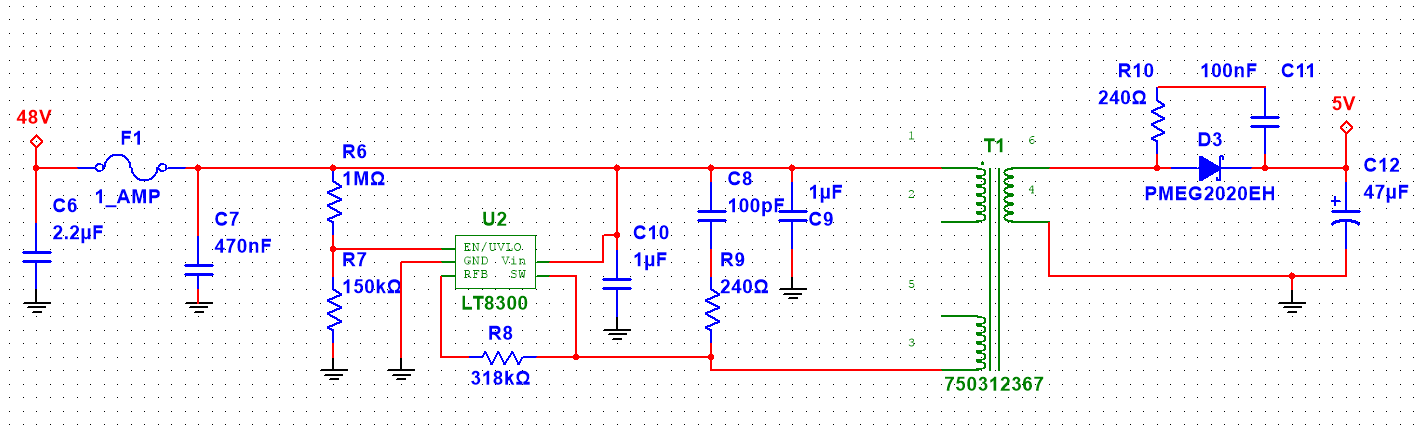
\includegraphics[width=0.7\linewidth]{Hardware/Pictures/SMPS_hw}
	\caption{SMPS hardware overview}
	\label{fig:SMPS_control}
\end{figure}

\subsection{Implementation}
It has been chosen to use the LT8300 Isolated Flyback Converter. The implementation is done almost according to the datasheet except there is implemented a snubbercircuit and a decoupling before the transformer.  \\

There is various resistors can be changed and thereby change the different things e.g. the output voltage. 

The value of the resistor R8 on figure \ref{fig:SMPS_control} is calculated on the formula below.

\begin{align}
	\begin{split}
		I_b &= \frac{N*(V_{out}+V_F)}{100$\my$A}
	\end{split}
\end{align}

Where:\\
N is the number of turns on the primary inductor. \\
$V_{out}$ is the desired output voltage from the SMPS. \\
$V_F$ is the forward voltage of the diode in output stage. \\

\subsection{Unity test}
text